\section[Kommunikation (Benjamin Brandt, Christopher Althaus)]{Kommunikation\begin{tiny} (Benjamin Brandt)\end{tiny}}\label{sec:communication}
Die Kommunikation der App mit dem Server läuft bei der Kommunikation der App mit dem RESTful Webservice über Http Befehle und für das Senden von Alarmnachrichten an die verschiedenen Geräte  wird Google Cloud Messaging verwendet.
\subsection{Google Cloud Messaging}
Der Service Google Cloud Messaging (GCM) wird Entwicklern von Android Apps kostenlos von Google zur Verfügung gestellt. Er erlaubt diesen über bestehende Google Server Infrastruktur Daten an ihre Apps  und von diesen an ihren Server zu senden. Hierbei übernimmt der GCM Service alle Aufgaben die mit der Übermittlung  der Nachricht zu tun haben.\\

Hier eine Auflistung der Hauptfunktionen von GCM:

\begin{itemize}
	\item Senden von Nachrichten vom eigenen Server zu den Nutzergeräten
	\item Empfangen von Nachrichten der Nutzergeräte am Server
	\item Die App muss nicht laufen um Nachrichten zu empfangen
	\item Es gibt keine grafische Oberfläche sämtliche Aufgaben die mit der Nachricht zusammenhängen werden von der eigenen Anwendung gesteuert.
	\item Voraussetzung ist Android 2.2 Froyo mit installiertem Playstore
\end{itemize}
\newpage
\subsubsection{Architektur}
Die Architektur von Google Cloud Messaging  teilt sich in drei Bereiche auf. Der erste sind die GCM Connection Server die die Nachrichten von den Servern des Entwicklers annehmen und diese an die Android App des Benutzers schicken. Der zweite Bereich ist der Server des Entwicklers der die Nachrichten für die Benutzer Apps an die Connection Server sendet. Als dritter Bereich natürlich die Benutzer-App die sich zum Empfang von GCM Nachrichten bei GCM registrieren muss um eine eindeutige ID zu erhalten und dadurch nur für sie bestimmte  Nachrichten erhält.\\

\begin{figure}[H]
\centering
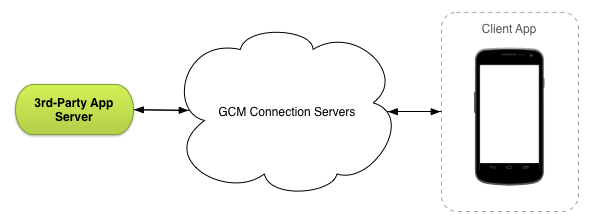
\includegraphics[width=\textwidth]{/GCMstruktur.png}
\caption{Struktur von GCM}
\label{fig:GCMstrukutr}
\end{figure}
\subsubsection{GCM Connection Servers    (Christopher Althaus)}
Die Kommunikation mit dem GCM Connection Server kann mittels den zwei Kommunikationsprotokollen HTTP und XMPP (Extensible Messaging and Presence Protocol) stattfinden. Mit Hilfe von XMPP kann eine bidirektionale Verbindung vom Client zum Server erfolgen, während mittels HTTP lediglich Daten vom Server an den Client (Android Gerät) übertragen werden können.\\
Wie bereits beschrieben, wird sämtliche Kommunikation der App mit Hilfe von HTTP realisiert und lediglich die Alarmnachrichten sollen mittels GCM an den Client übertragen werden. Da hierfür keine bidirektionale Verbindung notwendig ist und sich die Implementierung des XMPP Protokolls sowohl Client- als auch Serverseitig wesentlich aufwändiger gestaltet als die des HTTP Protokolls, ist entschieden worden für die GCM Kommunikation das HTTP Protokoll einzusetzen. 
\subsubsection{Android    (Original: Benjamin Brandt, Überarbeitet: Christopher Althaus)}
Wie bereits beschrieben, liegt der Vorteil der Nutzung des GCM Services unter Android darin, dass keine zusätzliche Verbindung überwacht werden muss. Das schont zum einen die Akkulaufzeit und erspart zum anderen die Implementierung eines Dienstes, der ständig eine Verbindung mit dem Server herstellt.\\
Geht eine Alarmnachricht unter Android ein, wird vom Google Service ein Broadcast ausgelöst. Innerhalb der App wird mittels eines \textit{Broadcast Receivers} auf solche Broadcasts gewartet. Geht beim \textit{Boradcast Receiver} eine GCM Nachricht ein, so wird ein Service aufgerufen, der diese auswertet. Grundsätzlich können die drei Nachrichtentypen \textit{SEND\_ERROR}, \textit{DELETED} und \textit{MESSAGE} auftreten. Nachrichten vom Typ \textit{MESSAGE} werden von der App weiterverarbeitet. Bei den anderen beiden Typen handelt es sich um Fehler, welche lediglich zur Fehleranalyse im Log festgehalten werden.\\
Geht eine GCM Nachricht vom Typ \textit{MESSAGE} ein, so wird automatisch davon ausgegangen, dass es sich um eine Alarmnachricht vom Server handelt, da der GCM Service innerhalb der App lediglich hierfür benutzt wird. Als Resultat wird die Alarmierung des Nutzers gestartet. Die dazu genutzte Methode ist zum besseren Verständnis im Listing \ref{lst:GCMAlarm} aufgeführt.
\begin{lstlisting}[caption={Senden von Nachrichten vom Server},label=lst:GCMAlarm]
 public static void sendAlarmNotification(Context context, String msg) {
   NotificationManager mNotificationManager = (NotificationManager)context.getSystemService(Context.NOTIFICATION_SERVICE);
   PendingIntent contentIntent = PendingIntent.getActivity(context, 0, new Intent(context, Info.class), 0);

   NotificationCompat.Builder mBuilder = new NotificationCompat.Builder(context)
     .setSmallIcon(R.drawable.icon)
     .setContentTitle("QuakeDetec")
     .setStyle(new NotificationCompat.BigTextStyle()
     .bigText(msg))
     .setContentText(msg);
     
   if(vibrationActivated)
      mBuilder.setVibrate(new long[]{0,300,100,300,100,300,100,300,100,300,100});
   if(soundActivated)
      mBuilder.setSound(Uri.parse("android.resource://" + context.getPackageName() + "/" + R.raw.alarm));
	
   mBuilder.setContentIntent(contentIntent);
   mNotificationManager.notify(1, mBuilder.build());     
 }
\end{lstlisting}
Wie im Quellcodeauszug ersichtlich, erfolgt die Alarmierung des Nutzers auf drei verschiedene Weisen. Zum einen wird eine Benachrichtigung innerhalb der Taskbar angezeigt. Diese Benachrichtigung enthält als Text die Nachricht, die der Server beim Auslösen des Alarms mitschickt. Dabei handelt es sich um Informationen, die das erkannte Erdbeben betreffen. Zusätzlich wird, falls der Vibrationsmotor des Handys nicht deaktiviert ist, ein Vibrationsalarm ausgelöst. Zudem wird für den Fall, dass das Gerät nicht auf lautlos geschaltet ist, ein Alarmton wiedergegeben.\\
Zum Auslösen des Alarms wird die Klasse \textit{NotificationManger} genutzt. Diese ist innerhalb von Android für jegliche Art der Benutzerbenachrichtigung zuständig.


\subsubsection{Server}
Der Server sendet eine Benachrichtigung an die GCM Server diese leiten die Nachricht an die betroffenen Geräte-IDs weiter. Dies wird über einen REST-Methodenaufruf durchgeführt. Dieser wird an die Adresse https://android.googleapis.com/gcm/send gesendet, die Nachricht ist mit einem Authorisationskey ausgestattet damit nur Nachrichten vom richtigen Server gesendet werden können. Der zugehörige Programmcode ist unter \ref{ServerSeGCM} abgebildet.

\begin{lstlisting}[caption={Senden von Nachrichten vom Server},label=lst:ServerSeGCM]

URL url = new URL(this.configuration.getApiUrl());
			HttpURLConnection http = (HttpURLConnection) url.openConnection();
			http.setDoOutput(true);
			http.setRequestMethod("POST");
			http.setRequestProperty("Content-Type", "application/json");
			http.setRequestProperty("Authorization", "key="+this.configuration.getAuthorizationKey()); //
			
			OutputStreamWriter writer = new OutputStreamWriter(http.getOutputStream());
			writer.write(rawData.toString());
			writer.flush();

\end{lstlisting}

Der Server empfängt wie unter \ref{lst:ServerEmGCM} aufgelistet, auserdem eine Bestätigung der Zustellung von den GCM Servern, diese enthält eine Zahl die koodiert ob die Nachricht angekommen und richtig interpretiert wurde. Bei Erfolg wird die Nachricht mit Code 200 bestätigt. Bei einer JSON Nachricht kann auch der Code 400 gesendet werden wenn z.B. ein anderer Datentyp als erwartet gesendet wurde. Wenn der Code 401 gesendet wird, ist die Authentifizierung am GCM Server nicht mit Erfolg abgeschlossen worden. Hiermit wird sichergestellt das Nachrichten nur vom richtigen Server gesendet werden können. 


\begin{lstlisting}[caption={Empfangen von Bestätigungen am Server},label=lst:ServerEmGCM]

BufferedReader reader = new BufferedReader(new InputStreamReader(http.getInputStream()));
			StringBuilder result = new StringBuilder();
			
			for (String line; (line = reader.readLine()) != null; ) {
				result.append(line);
			}

			writer.close();
			reader.close();

\end{lstlisting}
